\documentclass[11pt]{report}
\bibliographystyle{ieeetr}
\usepackage[a4paper, total={6in, 8in}]{geometry}
\usepackage{amsmath}
\usepackage{blindtext}
\usepackage{parskip}
\usepackage{enumitem}
\usepackage[nottoc,numbib]{tocbibind}
\usepackage[section]{placeins}
\usepackage{graphicx} % Required for inserting images
\usepackage[english]{babel}
\usepackage{pdfpages}
\usepackage{xargs}                      % Use more than one optional parameter in a new commands
%\usepackage[pdftex,dvipsnames]{xcolor}  % Coloured text etc.
%
\usepackage[colorinlistoftodos,prependcaption,textsize=tiny]{todonotes}
\newcommandx{\unsure}[2][1=]{\todo[linecolor=red,backgroundcolor=red!25,bordercolor=red,#1]{#2}}
\newcommandx{\change}[2][1=]{\todo[linecolor=blue,backgroundcolor=blue!25,bordercolor=blue,#1]{#2}}
\newcommandx{\info}[2][1=]{\todo[linecolor=OliveGreen,backgroundcolor=OliveGreen!25,bordercolor=OliveGreen,#1]{#2}}
\newcommandx{\improvement}[2][1=]{\todo[linecolor=orange,backgroundcolor=orange!25,bordercolor=orange,#1]{#2}}
\newcommandx{\thiswillnotshow}[2][1=]{\todo[disable,#1]{#2}}

\usepackage{acro}
\usepackage[colorlinks=false]{hyperref}
\usepackage{pdfcomment}

\acsetup{
	make-links 		= 	false,
	pdfcomments/use		=	true,
}

\DeclareAcronym{VTC}{short = {VTC}, long = {Value-transfer chain}, pdfcomment = {Value-transfer chain}}

\DeclareAcronym{GPC}{short = {GPC}, long = {General-purpose chain}, pdfcomment = {General-purpose chain}}
\DeclareAcronym{ESG}{short = {ESG}, long = {Environmental Social \& Governance}, pdfcomment = {Environmental Social \& Governance}}



\parskip 2ex
\parindent 0pt

\title{GreenBlocks - SMT PdM}
\author{mbelanger.poly}
\date{August 2023}


\begin{document}

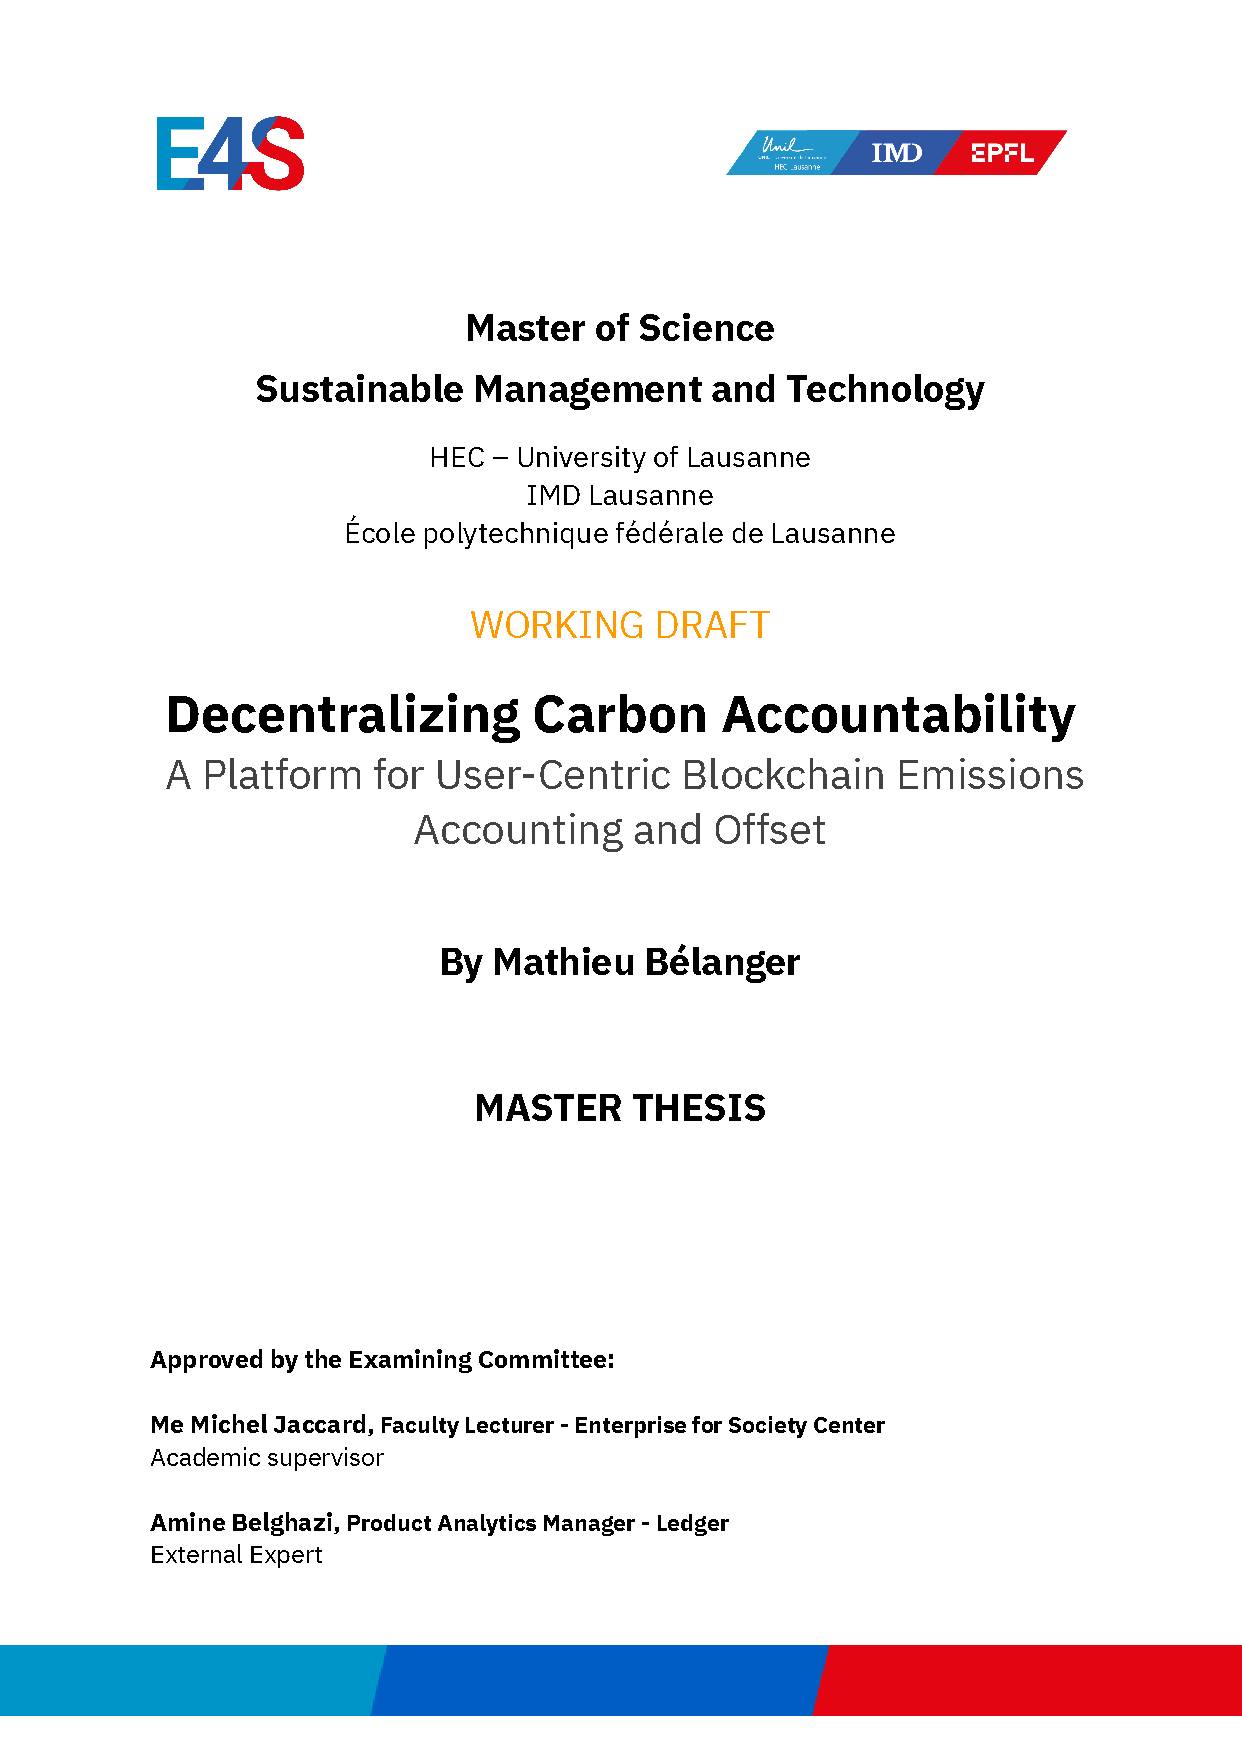
\includepdf[pages={1-2}]{cover.pdf}
\section*{Abstract}
\change{Put abstract in e4s template}
\improvement{Is this too long?}

Executive summary.
The advent of blockchain technology has raised concerns about its high energy use and carbon emissions. This is partly due to the current dominance of proof-of-work-driven Bitcoin, the first network to gain widespread adoption and media coverage. However, different consensus mechanisms and design choices result in varying environmental footprints across blockchains. While the recent release of the first industry blockchain \acp{ESG} benchmark enables standardized comparisons between chains at an aggregate level, a granular methodology for user-level emissions accounting is lacking. \ac{ESG} \

This thesis introduces an attribution model designed to map the carbon footprint of blockchain at a user-responsibility level. Novel to this research is the attempt to weigh responsibility factors based on the principle of proportional benefits. This approach exploits the inherent transparency of blockchain data to capture the relative value, specific to each network, that users place on different blockchain functionalities. We find that two generalizable categories of benefits emerge: the Transactional use case (benefits from active transacting or interacting) and the Asset-Securing use case (benefits from passively holding or securing assets). Key parameters such as asset balance, signed transactions, and gas expenditure are used as representative indicators of benefiting from a network use case. This methodology allocates the overall chain emissions to specific users based on their interaction patterns. The evolutions of network-specific transaction fees and market capitalization are used to derive weight for these parameters.

\improvement{Unsure. Is the part clear?}

Furthermore, a proof-of-concept tool (GreenBlocks) is built to showcase the attribution model, allowing users to estimate and offset their emissions through carbon credits. Based on the Ledger Live platform, this platform interacts seamlessly with leading blockchains and links with on-chain carbon market partners to retire offsets with maximal transparency.

Greenblocks provides transparent and personalized insights into blockchain emissions for end-users. By linking usage to quantified environmental impact, it promotes awareness. It enables offsets as a means for users to bear the actual costs behind the benefits they reap from using the technology. Moreover, it demonstrates the potential for on-chain data to be used as the foundation for an appropriately nuanced attribution of external costs in a system. Moving past rudimentary address metrics, more complex behaviors and benefits can be modeled, enabling the distribution of externalities like a Pigouvian tax. Thus, this thesis proposes a bottom-up, user-focused approach to align blockchain adoption with environmental sustainability. This is achieved by pioneering user-level footprint attribution, arising from the \textit{Benefiiciary pays principle}.


\change{Add section on further opportunities for the blockchain-sustainability space}

\newpage
\section*{Acknowledgements}
\tableofcontents



\chapter{Introduction}

\section{Background and Motivation}
\improvement{Compartiment in subsections to improve narrative flow}
\subsubsection*{Origins, promise and challenges of blockchain technology}
The advent of blockchain technology since the launch of Bitcoin in 2009 has sparked a revolution in systems of value transfer, transparency, and decentralization \cite{nakamotoBitcoinPeertopeerElectronic2008}. However, the early meteoric rise of cryptocurrencies and underlying blockchain networks has raised critical concerns regarding their environmental sustainability. With the benefit of hindsight, we can view this period as Gartner's Peak of Inflated Expectations. Now, with notorious founders imprisoned, increasing regulatory scrutiny, and the total cryptocurrency market capitalization down
XX\% from its peak \change{cite}, the blockchain ecosystem stands at a crossroads. This is an opportunity to refocus on the core propositions of blockchain technology and ensure its long-term viability.


The dominant network, Bitcoin, which utilizes a computationally-intensive proof-of-work consensus mechanism, has attracted particular scrutiny for its high energy consumption. Recent estimates indicate the Bitcoin network alone may consume between 115 and 150 TWh annually, comparable to entire countries like the Netherlands \cite{devriesRevisitingBitcoinCarbon2022,neumuellerCambridgeBitcoinElectricity2021}. This growing apetite for energy competes with the just starting energy transition, putting electrical production and distribution networks under stress. Finally it also results in significant CO2 emissions, hardly compatible with global climate goals like the Paris Climate Accords.

\subsubsection*{Limitations of current approaches}
However, we must recognize the complexity and nuance when evaluating blockchain sustainability. Consensus protocols, design choices, and use cases vary greatly across different networks, leading to wide variability in energy needs and emissions. For instance, proof-of-stake networks like Cardano and Solana promise energy savings by factors of 1000x or more compared to proof-of-work \cite{kohliAnalysisEnergyConsumption2023}. Moreover, Ethereum recently completed its highly anticipated, technically and politically complex transition from proof-of-work to proof-of-stake, demonstrating that such migrations are viable for major networks. \cite{EthereumMergeYour2022} The nascent field of blockchain sustainability analysis must evolve more granular, differentiated perspectives.

Initial responses from the blockchain industry have focused on high-level aggregate comparisons and rankings between networks. For example, recent benchmarks like the Crypto Carbon Ratings Institute methodology provide standardized comparisons of the total lifecycle emissions across chains [5]. However, these overlook the diversity of users and fail to provide accountability at an individual level.

This poses a critical gap, especially as blockchain technology expands into mainstream adoption. We lack a methodology to attribute network-wide emissions to specific users based on their unique activity patterns and values. Such granular carbon accounting can raise awareness of individual impact and empower ethical participation.

\subsubsection*{Opportunities for user-level footprinting}

To address this, the novel approach in this thesis involves an attribution model that weighs factors like asset holdings, transactions, and computations based on their estimated importance to users on each chain. By considering relative user perspectives, we can map emissions more accurately to individual entities like protocols, DAOs, or end-users. This unconventional yet powerful approach unlocks new potentials for transparency, responsibility, and sustainability.

\section{Problem Statement}

As blockchain technology progresses into mainstream integration, the lack of transparency and accountability for emissions at an individual user level poses a critical gap. For example, retail investors drawn to crypto assets may be unaware of the passive environmental impacts associated with their portfolios over time. There is also increasing offering of decentralized applications (web3) with usage beyond those of investing. Granular carbon accounting and attribution to individual wallets can raise awareness and enable offsetting as a means for users to take responsibility of their actions.

Moreover, this gap becomes even more complex for providers of decentralized apps or decentralized autonomous organizations (DAOs) comprising multiple smart contracts and user addresses. Without a methodology for attributing network-wide emissions based on collective usage patterns, a DAO cannot fully assess and mitigate its overall carbon footprint.

Therefore, the overarching problem this thesis addresses is:

"How can we design an attribution model that allocates the carbon emissions of any blockchain network to specific user entities or addresses in a transparent, accurate, and relevant manner based on their unique activity patterns?"


\section{Research Questions and Ojbectives}

To systematically address the problem of transparent and accurate carbon attribution for blockchain users and entities, this thesis pursues four key research questions:

\begin{enumerate}
    \item How can blockchain emission factors be quantified at a granular, user-centric level, beyond aggregate network-wide estimates?
    \item What are appropriate metrics and weighting systems to reflect the responsibilities of diverse blockchain users based on their activities?
    \item How can we validate and demonstrate such an attribution model through a practical implementation?
    \item What are the broader implications of user-centric emissions accounting for accelerating sustainability as blockchain technology matures?
\end{enumerate}

The main objectives of this work are:

\begin{description}

    \item [Develop a User-Level Attribution Model] \hfill \\
          Develop a robust emissions attribution methodology based on usage and responsibility.
    \item [Greenblock: Pratical Application] \hfill \\
          Implement and validate the model through a functional proof-of-concept application.
    \item [Promote awareness and Responsibility] \hfill \\
          of environmental impact among blockchain users.
    \item [The Future of Sustainability and Blockchain] \change{to complete}
\end{description}

\section{Scope and Limitations}
TO COMPLETE


\section{Structure of the Thesis}
TO COMPLETE

\chapter{Litterature Review}
\section{Economic Externalities}
\section{Evolution of Blockchain Technology}
\section{Environmental Impact of Blockchains}
\subsection{Energy Consumption and Related Emissions}
\subsection{Current Measurement Methodologies and Datasets}
\section{User-Level Emissions Attribution}


\chapter{Methodology: User-Level Emissions Attribution Model}
\section{Overview}

\todo{Find where to include steps of the work. Interviews and data collection}

As blockchain technology expands onto more use cases and scale in it adoption, quantifying and attributing associated carbon emissions transparently emerges as a valid need. While aggregate estimates provide high-level network overviews, they fail to offer accountability at an individual user level, posing a user education gap and potentially a product need.

This chapter introduces a novel methodology to attribute network emissions to specific blockchain addresses based on proportional benefits gained by users. By mapping network footprints to end-users, protocols, and DAOs, this framework enables entities to understand, report, and take action based on their responsibility in the overall emissions.

The methodology is underpinned by ethical and economic theories suggesting emissions be allocated based on the proportional benefits users derive, both actively through transferring value and interacting, and passively from securing assets. Historical trends in activity metrics like fees and market value provide useful signals into evolving blockchain utility dynamics and user perceptions of value.

By incorporating these perspectives, the model aims for a fair, customizable attribution aligned with the real-world value users obtain from blockchain networks. The following sections detail this approach and rationale.

\section{Background - Emission attribution considerations}

\subsection{Blockchain Typology}
Blockchains can be categorized into two main types based on their primary function and underlying mechanics:
\improvement{this separation is also justified by the polluter and beneficiary pays framework. The limited ressource (blockspace) is shared differently for bitcoin and ethereum}

\begin{description}
    \item[\ac{VTC}] Chains that focus on transferring assets between addresses (e.g. Bitcoin and derived). VTCs are focused primarily on enabling value transfers through native cryptocurrency tokens. These chains do not typically support complex smart contract functionality like GPCs or make similar functionalities unergonomic to implement. The key operational metric for VTCs is the transaction throughput, constrained by blocksize and block intervals.

    \item[\ac{GPC}] Chains that allow the deployment of smart contracts and decentralized applications (dApps) in addition to value transfer (e.g. Ethereum, Cardano, Solana). On these networks, transactions and computations are quantified using a metric called gas\footnote{See: https://ethereum.org/en/developers/docs/gas/}. This concept was introduced by Vitalik Buterin in Ethereum's initial whitepaper \cite{buterinEthereumNextgenerationSmart} as a means to disincentivize computationally intensive smart contracts that could clog the network. Gas puts a cost on network utilization for activities like executing code, storing data, or transferring tokens based on their computation complexity. This makes it more costly to interact with complex applications and prevents situations that would halt the network like an infinite loop in a smart contract.
\end{description}

Due to these fundamental differences, GPCs and VTCs require distinct approaches for carbon accounting. On VTCs, the limited blockspace is the bottleneck for transactions. Hence, users conducting more transactions take up a greater share of blockspace and have higher responsibility for the chain's emissions. On GPCs, gas expenditure more accurately reflects utilization and impact on the network's computation and storage load. Users spending more gas have a greater share of responsibility by consuming more of the network's resources and throughput capacity.

Existing studies have estimated blockchain emissions using aggregate network energy use or miner rewards \cite{devriesCryptocurrenciesRoadSustainability2022,devriesRevisitingBitcoinCarbon2022,neumuellerCambridgeBitcoinElectricity2021,mcdonaldEthereumEmissionsBottomup2022}. However, these top-down approaches fail to capture user behavior and responsibility. Our methodology addresses this limitation through a transparent attribution model tailored to GPCs and VTCs using usage factors like gas and transactions. The following sections detail this framework.

\subsection{Attribution framework}
\improvement{To review!! Add share infrastructure metaphor. Introduce polluter/benef pays from the litt review.}
The Need for Proportional Benefit Attribution
Carbon emissions from blockchain operations should not only be tied to direct causative actions (polluter pays principle) but also to the benefits derived from these actions (beneficiary pays principle). The synthesis of the polluter pays and beneficiary pays principles results in a more nuanced understanding of emission responsibility.

\subsubsection*{Transactional Activities}

Direct Actions and Associated Benefits
Signing transactions or spending gas actively utilizes block space, which is a limited resource. This not only results in emissions but is also a direct reflection of users seeking to derive transactional benefits from the blockchain. By engaging in these activities, users are both contributing to emissions and benefiting from the network's utility.

\subsubsection*{Beyond Transactions: Passive Utility and Continuous Benefit}
While active behaviors like transactions and gas spending are evident, there exists a passive benefit that users gain simply by holding assets on the network. This benefit accrues continuously over time and is inherently dependent on the active behaviors of others. Passive holders derive benefits from the blockchain's ability to secure value, which goes beyond the direct actions of signing transactions or spending gas. This implies an added layer of responsibility that isn't captured by looking at transactions alone.

\subsubsection*{Balancing the Attribution: Weighing Active and Passive Benefits}
With two distinct parameters (active transactions/gas spending and passive holding of value), there's a need to determine their respective weights in the attribution formula. The conjunction of the polluter pays and beneficiary pays principles demands an understanding of the relative utility of both active and passive benefits to users.

\subsubsection*{Deriving Weights Factors: The Role of Transaction Fees and Market Capitalization}
To establish the relative importance of active versus passive benefits, historical trends of transaction fees and market capitalization serve as proxies. These indicators reflect user-perceived utility and importance of both types of benefits over time. Transaction fees offer insights into the value users associate with active transactional capabilities, while market cap reflects the trust and perceived security in the network's ability to hold value. These can be used to derive dynamic weights for the two parameters in the emission attribution formula.



\subsubsection*{On Including Passive Holdings as a Responsibility parameter}
A key diffentiator is the inclusion of historical balance as a responsibility factor. Traditionally, emissions accounting ties responsibility to direct actions like executing transactions or computations. \improvement{Add metaphore of traditionnal infrastructure. Roads and km usage vs passive benefit of the road proximity} However, in blockchains, holding assets passively (function of preserving/securing value) also necessitates ongoing mining and transaction fees payed by transacting users, in order to preserve liquidity and value.

\improvement{Put justifications in list form to emphasize each point}

Specifically, continuous mining activity and block creation are critical to maintain an active market and allow holders to liquidate assets. This activity is incentivized through transaction fees. Higher fees increase miner rewards, resulting in greater security and liquidity that benefit holders.

Therefore, despite no active behavior, holding blockchain assets creates latent demand for emissions-intensive mining. Considering this relationship, the attribution model argues for allocating part of emission responsibility to asset holders, or more generally how intensively a use is using the blockchain function of securing value.

\section{Model Components}

Building on the previous overview, this section details the specific components of the emission attribution model.

\subsection{Historical Blockchain Emissions Data}
\todo{expand, explain LCA amortized emissions}
The emission rate \(E(\tau)\) represents the overall amount of tCO2-equivalent emissions generated by a blockchain at time $\tau$. This is chain-specific, with data aggregated from existing studies \cite{neumuellerCambridgeBitcoinElectricity2021,stollCarbonFootprintBitcoin2019}.

\begin{equation}
    E(\tau) = \text{Emission rate of chain $s$ at time $\tau$}
    \label{eq:emission_rate}
\end{equation}

\todo{Detail combination of papers and dataset access}

\subsection{User Attribution Parameters}

The attribution share ($S$) for an address owned by a user is proportional to the measurement of two categories of behavior-benefits. Interactve behavior ($I$), directly responsible for a share of emissions and reaping direct benefits from the network interaction; and Passive behavior ($P$), indirectly accruing benefits from the network's ongoing operation.

\begin{equation}
    S \propto (I + P)
    \label{eq:attribution_share}
\end{equation}

Interactive behavior is measured by the share of network ressources, blockspace, allocated to the user's address for his interactions during a period. For \ac{VTC}s, this is reported by the number of signed transactions, for \ac{GPC}s it is the sum of gas spent in signed transaction. Passive behavior is measured by the share of the total value secured by the network owned by the user's address.

The three factors are, for an address on a given chain and at period $\tau$:

\begin{description}[leftmargin=!, labelwidth=\widthof{\bfseries Passive Behavior}]

    \item[Interactive Behavior $(I)$] \hfill
        \begin{itemize}[labelwidth=4cm, align=left, labelsep=0pt]
            \item[\( T(\tau) = \frac{T_{addr}(\tau)}{T_{\text{total}}(\tau)} \)]
                Number of transactions signed by the adress as a percentage of total transactions (for VTCs).

            \item[\(G(\tau) = \frac{G_{addr}(\tau)}{G_{\text{total}}(\tau)} \)]
                Gas spent by the adress as percentage of total gas in blocks (for GPCs).
        \end{itemize}

    \item[Passive Behavior $P$] \hfil
        \begin{itemize}[labelwidth=4cm, align=left, labelsep=0pt]
            \item[\(B(\tau) = \frac{B_addr(\tau)}{B_{\text{total}}(\tau)} \)]
                Average adress Balance as a percentage of total token supply.
        \end{itemize}

\end{description}
\parsep 5pt
Thus from equation \eqref{eq:attribution_share} we have the chain-specific emission attribution share for an address at period $\tau$:


\begin{equation}
    S(\tau) \propto [B(\tau) + \begin{cases}
            T(\tau) & \text{for VTC} \\
            G(\tau) & \text{for GPC}
        \end{cases}]
    \label{eq:attribution_share_chain_type}
\end{equation}

\subsection{Weighting factors}


\improvement{Add formalisation of the weighting factors measurment. Maybe add a figure to illustrate the concept}

\subsection{Attributed Emissions}

Combining chain emission rate \eqref{eq:emission_rate}, the attribution parameters \eqref{eq:attribution_share_chain_type} and corresponsing weights (()), we get the the CO2e emissions \(A(\tau)\) attributed to an address on a given blockchain for the period $\tau$ general form:


\begin{align}
    A(\tau) = E(\tau) \times \left[\beta \cdot B(\tau) + \gamma \begin{cases}
                                                                        T(\tau) & \text{for VTCs} \\
                                                                        G(\tau) & \text{for GPCs}
                                                                    \end{cases}\right]
\end{align}

\begin{align}
    A(\tau) = E(\tau) \times \left[\begin{cases}
                                           \beta \cdot B(\tau) + \gamma T(\tau)  & \text{for VTCs} \\
                                           \beta \cdot B(\tau) +  \gamma G(\tau) & \text{for GPCs}
                                       \end{cases}\right]
\end{align}

%\begin{equation}
%    A_{s}(\tau) = E_{s}(\tau) \times
%    [
%        \alpha_{s}\frac{B_{\text{addr},s}(\tau)}{B_{\text{total},s}(\tau)} +
%        \beta_{s}  \frac{G_{\text{addr},s}(\tau)}{G_{\text{total},s}(\tau)} +
%        \gamma_{s} \frac{T_{\text{addr},s}(\tau)}{T_{\text{total},s}(\tau)}
%    ]
%\end{equation}


% \begin{equation}
%     A_{s}(\tau) = E_{s}(\tau) \times [\alpha_{s} B(\tau) + \beta_{s} G(\tau) + \gamma_{s} T(\tau)]
% \end{equation}

% Since we have $\beta_{s} = 0$ for VTCs and $\gamma_{s} = 0$ for GPCs, the attributed emissions on chain $s$ of type $|VTC, GPC|$ are:

% \begin{equation}
%     A_{VTCs}(\tau) = E_{s}(\tau) \times [\alpha_{s} B(\tau) + \beta_{s} G(\tau)]
% \end{equation}

% \begin{equation}
%     A_{GPCs}(\tau) = E_{s}(\tau) \times [\alpha_{s} B(\tau) + \beta_{s} G(\tau)]
% \end{equation}

% With $\alpha_{s} + \beta_{s} + \gamma_{s} = 1$ and $\alpha_{s}, \beta_{s}, \gamma_{s} \geq 0$.

\subsection*{Cumulative Emissions}

The cumulative emissions $C(t)$ for a user across a collection of owned adresses $S$ up to time $\tau$ is:

\begin{equation}
    C(t) = \sum_{s \in S} \int_{0}^{t} A_s(\tau) d\tau
\end{equation}

This aggregates the attributed emissions across chains over time. The next section concludes this methodology overview.

\section{Data Sources and Collection}
\section{Validation and Robustness Analysis}
\subsection{Approach to Validation}
\subsection{Sensitivity Analysis Design}

\chapter{Implementation: GreenBlocks Platform}
\section{Overview}
\begin{figure}[h!]
    \centering
    \centerline{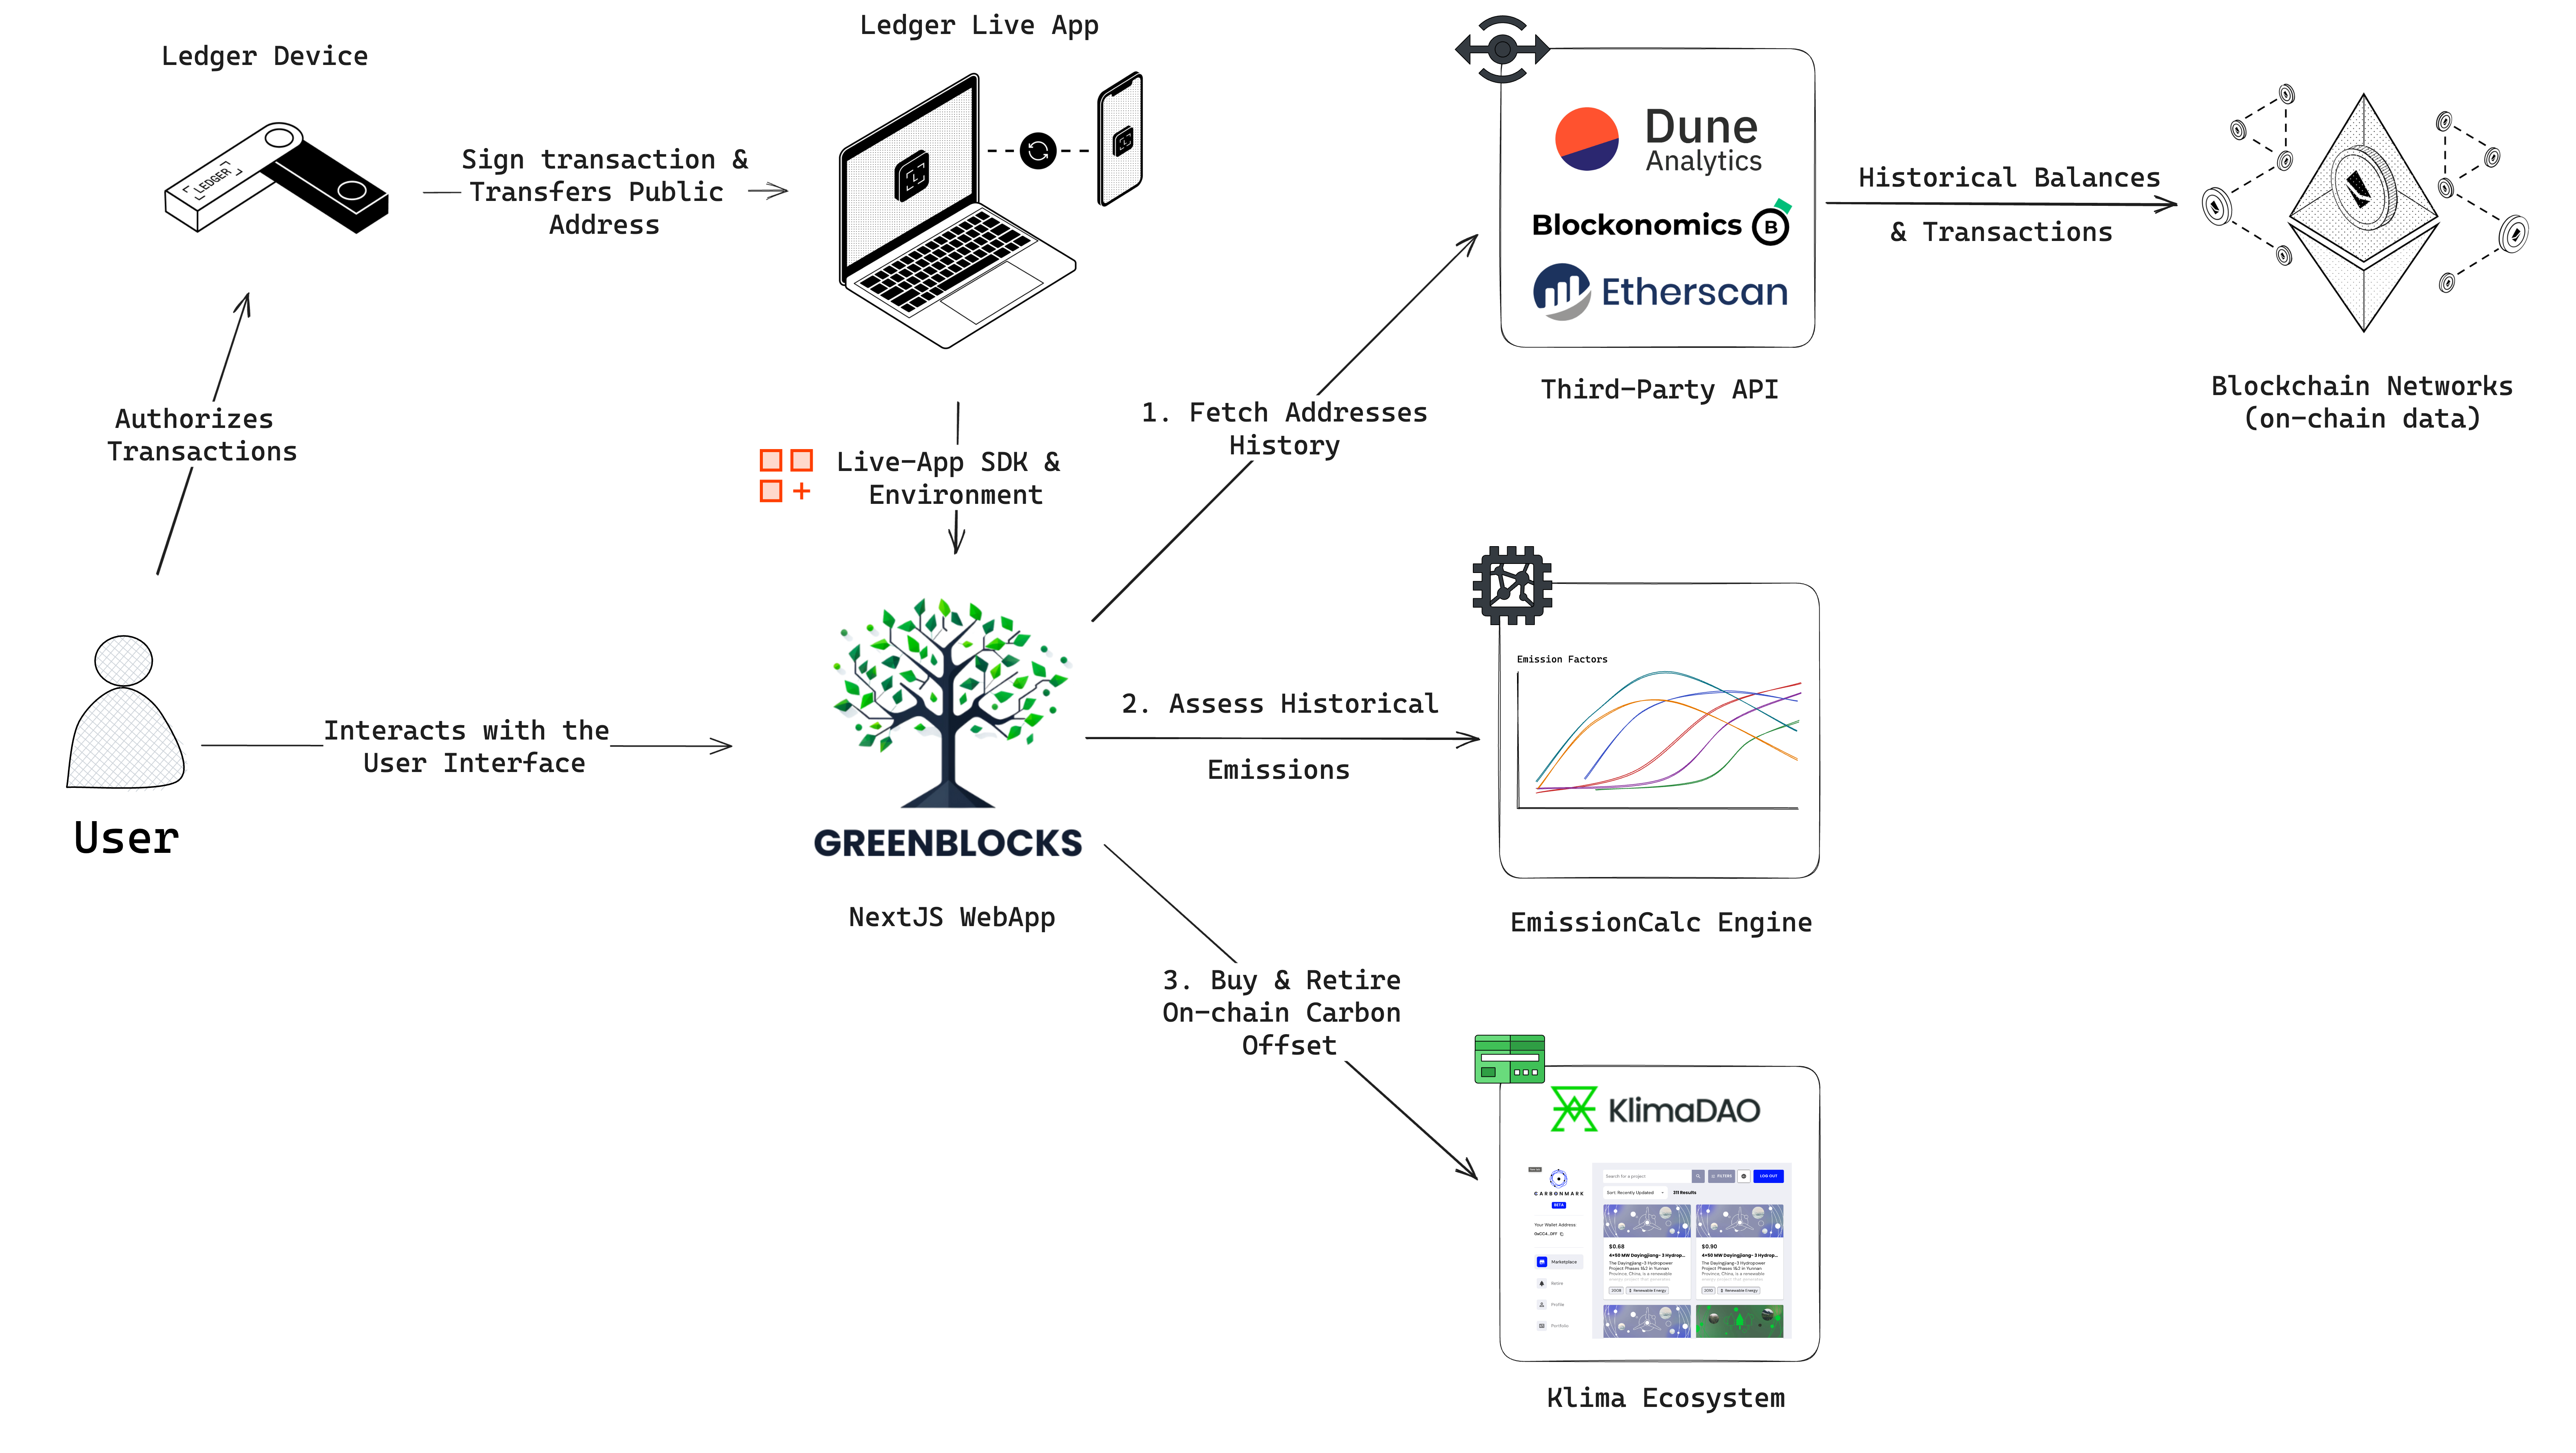
\includegraphics[scale=0.08]{figures/functionnal architecture.png}}
    \caption{GreenBlocks - Functionnal Architecture}
    \label{fig:functionnal_architecture}
\end{figure}

\begin{figure}[hbt!]
    \centering
    \centerline{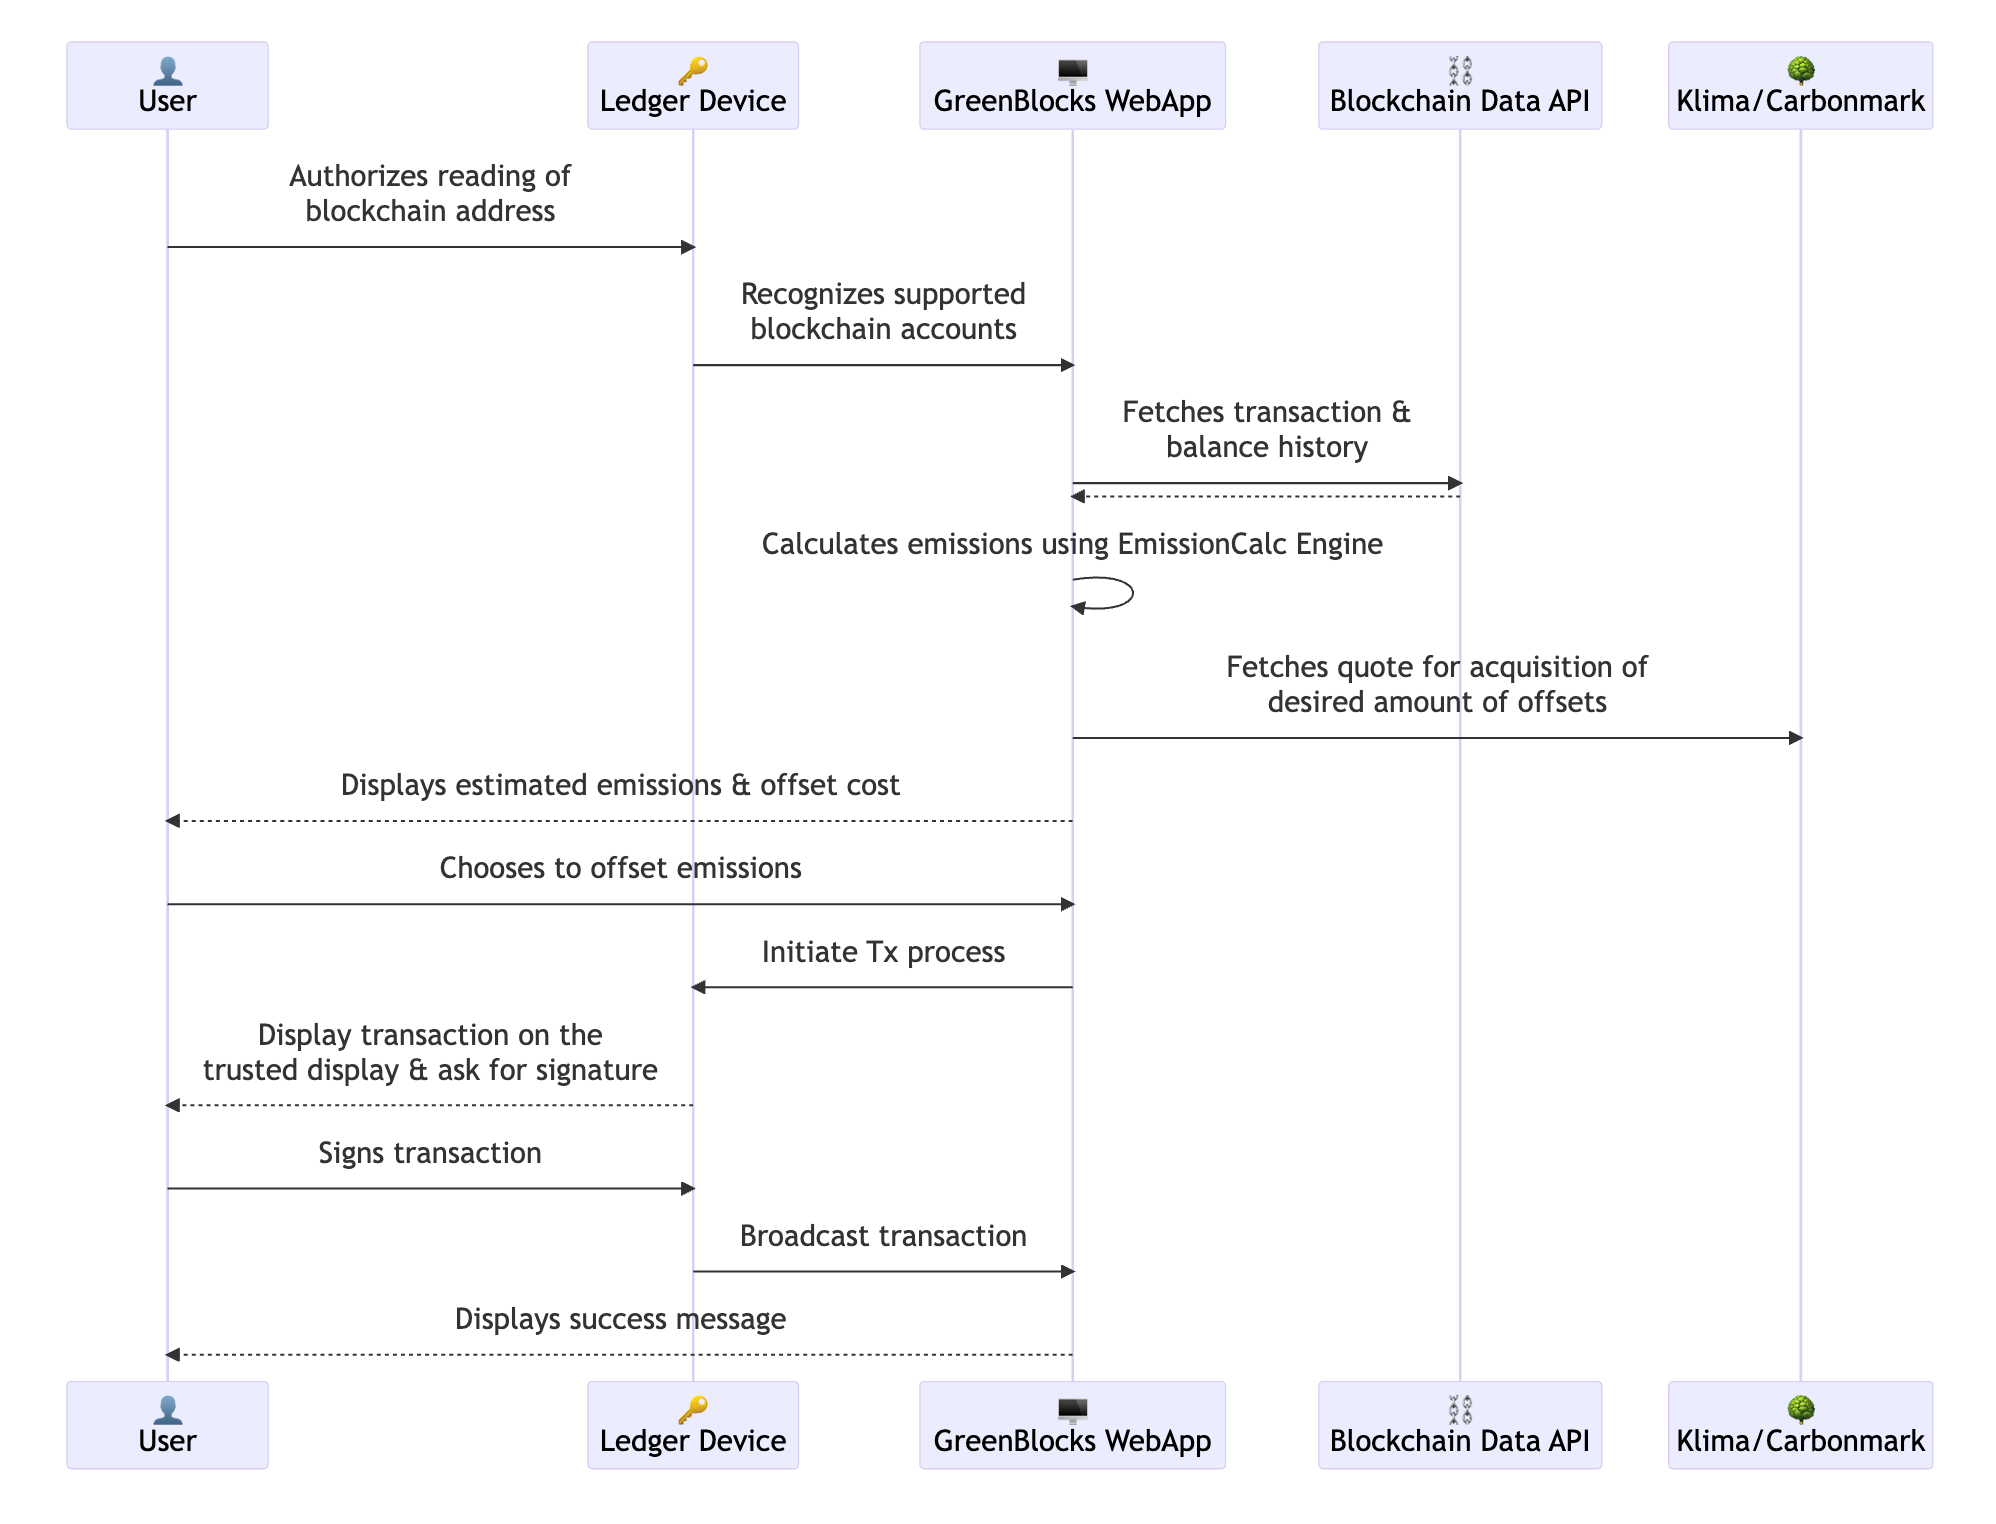
\includegraphics[scale=.27]{figures/sequence.png}}
    \caption{GreenBlocks - Sequence Diagram}
    \label{fig:sequence}
\end{figure}

\change{Review figure size for readability. Consider redo on lucid to control font}


\section{System Architecture and Components}
\subsection{User Interface Layer}
\subsection{Middleware Layer}
\subsection{Backend Layer}
\subsection{Data Layer}
\section{Development Process}

\chapter{Discussion}
\section{Results and Analysis}
\section{Comparative Analysis: Different User Profiles and Protocols}
\begin{enumerate}
    \item Bitcoin holder
    \item Bitcoin trader
    \item Ethereum holder
    \item Ethereum App user
    \item Ethereum only since merge (or show all using a time-series on emissions)
\end{enumerate}

\section{Statistical Analysis}
\todo{Statistical analysis of a random sample of addresses}
\unsure{will it be possible to get a sample of bitcoin xpub. Otherwise focus on ethereum analaysis before \& post merge}

\subsection{Validation and Sensitivity Analysis Results}
\subsubsection{Validation Results}
\subsubsection{Sensitivity Analysis Findings}

\section{Limitations and Future Work}
\section{Further Opportunities for Blockchain and Sustainability}

\chapter{Conclusion}


\bibliography{bibliography.bib}


\end{document}